\documentclass[10pt, compress]{beamer}
\usetheme{m}
\usepackage{booktabs}
\usepackage[ampersand]{easylist}
\usepackage{minted}
\usemintedstyle{manni}
\usepgfplotslibrary{dateplot}

\title{Satellid: Personal Knowledge Manager}
\subtitle{with Web Technologies}
\date{18 March 2015}
\author{Muhammad Haidar Hanif}
\institute{Informatics Engineering - Gunadarma University}

\begin{document}

% ============================================================

\maketitle

% ============================================================

\begin{frame}[fragile]
  \frametitle{Outline}

  \begin{description}
    \item[Introduction]%: Background, Problem Statements, Objectives, Scope
    \item[Literature Study]%: KMS, SDLC, Design Pattern, Database, Programming, Platform, Framework, Soft. Testing, SCM
    \item[Analysis \& Design]%: Target User, User Types, User Stories, Contextual System, Functionality Flow, App Architecture, User Interface \& Interaction
    \item[Implementation \& Testing]%: Agile Development, Code, Result, and Test
    \item[Conclusion \& Suggestion]
  \end{description}

\end{frame}

% ============================================================

\section{Introduction}

% ------------------------------------------------------------

\begin{frame}[fragile]

  \begin{center}
  There are tons of \alert{daily personal knowledge} that must be managed,
  but they can't be handled with regular tools.
  \end{center}

\end{frame}

% ------------------------------------------------------------

\begin{frame}[fragile]

  \begin{center}
  \alert{Daily personal knowledge} are things like details of:
  \begin{itemize} \itemsep0pt
    \item people profile and contacts
    \item list of organizations and companies
    \item glossary of definition
    \item hardware and software product listing
    \item publication of books or presentations
    \item known or visited places
    \item upcoming and attended events
    \item multimedia info such as music or video
    \item and lot of other miscellaneous things
  \end{itemize}

  \end{center}

\end{frame}

% ------------------------------------------------------------

\begin{frame}[fragile]

  \begin{center}
    There are a lot of tools and systems for each of them.

    \alert{Need for just a single system}
  \end{center}

\end{frame}

% ------------------------------------------------------------

\begin{frame}[fragile]

  \begin{center}
  How to manage those \alert{daily personal knowledge} with single system?
  % So how to manage those tons of daily personal knowledge we have with just a simple and single system of knowledge manager that implemented with Web technologies?
  \end{center}

\end{frame}

% ------------------------------------------------------------

\begin{frame}[fragile]
  \frametitle{Primary Background}

  Solve a problem around \alert{\emph{daily knowledge management}} \\
  with a system to make it more effective.

\end{frame}

% ------------------------------------------------------------

\begin{frame}[fragile]
  \frametitle{Primary Objective}

  Define and develop a knowledge manager called\\
  \alert{``Satellid knowledge manager''},
  that built using Web technologies.
  % utilize knowledge template which use context and structure, to store and managing personal daily knowledge.

\end{frame}

% ------------------------------------------------------------

\begin{frame}[fragile]
  \frametitle{Problem Definition}

  \begin{enumerate}
    \item How to manage tons of personal knowledge we have with just a simple and single system of knowledge manager?
    \item How can knowledge manager naturally structure the data into knowledge that has context?
  \end{enumerate}

\end{frame}

% ------------------------------------------------------------

\begin{frame}[fragile]
  \frametitle{Problem Scope}

  \begin{itemize} \itemsep0pt
    \item Create a \alert{\emph{simpler system}} to do daily knowledge management for personal use
    % with \alert{basic \textsc{browse, read, edit, add, delete} (BREAD) features}.
    \item The main methodologies are agile, MVP, and ATDD.
    \item The main technologies are MongoDB, JavaScript, and Meteor framework.
  \end{itemize}

\end{frame}

% ============================================================

\section{Literature Study}

% ------------------------------------------------------------

\begin{frame}[fragile]
  \frametitle{Knowledge Management System}

  Data-Information-Knoweldge-Wisdom (\alert{DIKW}),\\
  Knowledge Management System (\alert{KMS}),\\
  \alert{Personal Knowledge Manager}

\end{frame}

% ------------------------------------------------------------

\begin{frame}[fragile]
  \frametitle{Software Development Life Cycle (SDLC)}

  \alert{Agile} methodologies,\\
  Minimum Viable Product (\alert{MVP}),\\
  Acceptance Test Driven Development (\alert{ATDD})

\end{frame}

% ------------------------------------------------------------

\begin{frame}[fragile]
  \frametitle{Design Pattern}

  \textsc{browse, read, edit, add, delete} (\alert{BREAD}),\\
  simple interaction and interface design with mockup,\\
  Single Page Application (\alert{SPA})

\end{frame}

% ------------------------------------------------------------

\begin{frame}[fragile]
  \frametitle{Database}

  Document-based \alert{NoSQL} database called \alert{MongoDB}

\end{frame}

% ------------------------------------------------------------

\begin{frame}[fragile]
  \frametitle{Programming}

  With \alert{JavaScript} related technologies,\\
  build a Web application,\\
  that use full stack framework called \alert{Meteor}
  % full stack = frontend + backend

\end{frame}

% ============================================================

\section{Analysis \& Design}

% ------------------------------------------------------------

\begin{frame}[fragile]
  \frametitle{Satellid}

  \begin{figure}[ht]
    \centering
    
\includegraphics[width=8cm]{include/satellid-logo.png}
    \label{fig:satellid-logo}
  \end{figure}

\end{frame}

% ------------------------------------------------------------

\begin{frame}[fragile]
  \frametitle{Analysis}

    \begin{block}{Target user:}
      Person who frequently gather and need to manage their knowledge at almost everytime.
    \end{block}

\end{frame}

% ------------------------------------------------------------

\begin{frame}[fragile]
  \frametitle{Analysis}

    \begin{block}{User Types:}
      Regular person, researcher, engineer, developer, designer,\\
      information architect, event speaker, student, teacher,\\
      leader, collaborator, colleagues, recruiter, etc
    \end{block}

\end{frame}

% ------------------------------------------------------------

\begin{frame}[fragile]
  \frametitle{Design: Contextual System}

  \begin{figure}[ht]
    \centering
    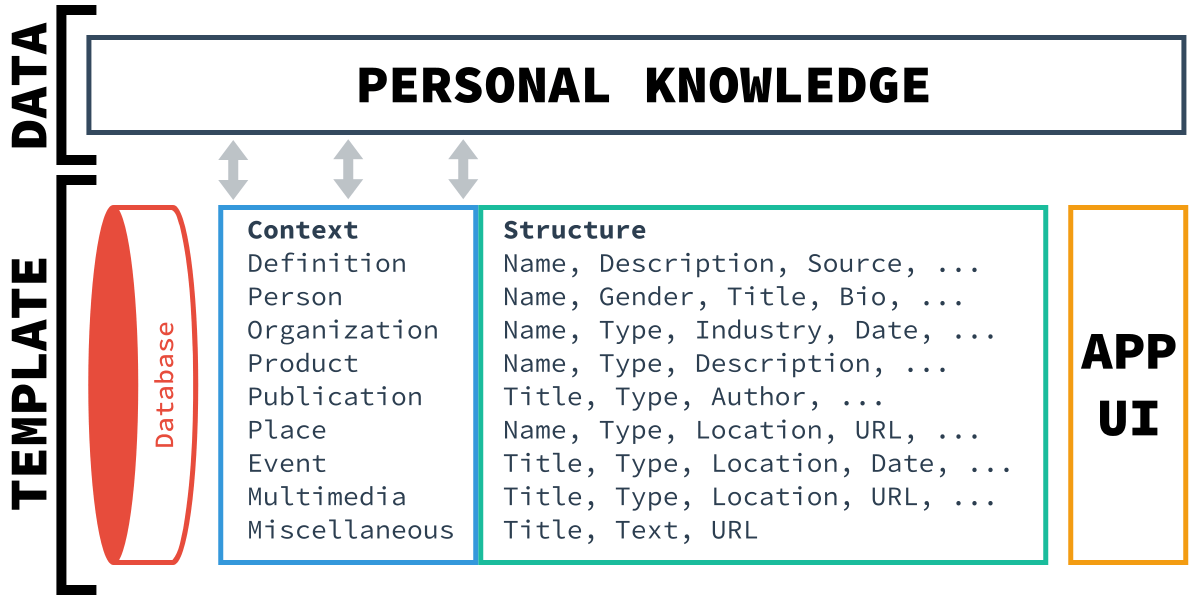
\includegraphics[width=9cm]{include/satellid-contextual.png}
    \caption{A data and template approach to classify the knowledge with its context and structure.}
    \label{fig:satellid-contextual}
  \end{figure}

\end{frame}

% ------------------------------------------------------------

\begin{frame}[fragile]
  \frametitle{Design: Application Architecture}

  \begin{figure}[ht]
    \centering
    \vspace{-25pt}
    %TODO
    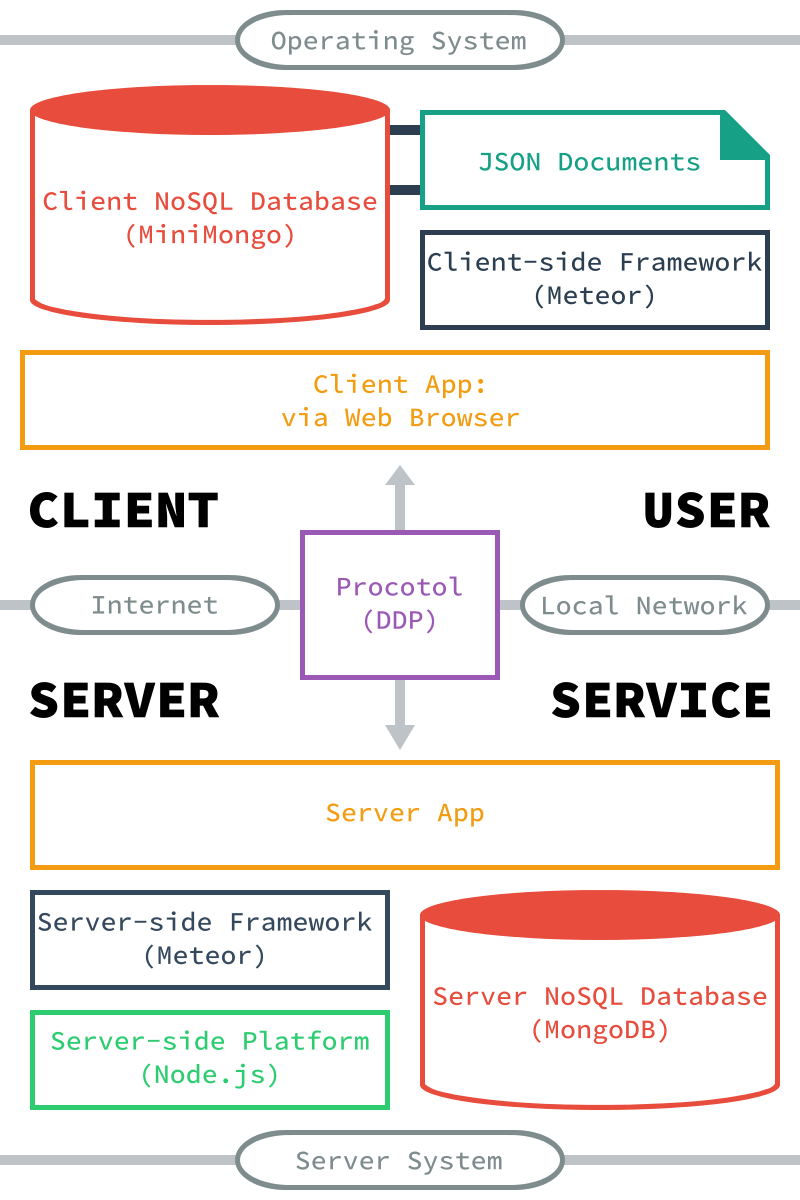
\includegraphics[height=8.5cm]{include/satellid-app-arch.png}
    \vspace{-10pt}
    \caption{Application Architecture}
    \label{fig:satellid-app-arch}
  \end{figure}

\end{frame}

% ============================================================

\section{Implementation \& Testing}

% ------------------------------------------------------------

\begin{frame}[fragile]
  \frametitle{Implementation: Code}

  Snippets of Server Code
  \begin{minted}[fontsize=\small]{javascript}
    if (Meteor.isServer) {
      Meteor.startup(function() {
        ...
      });
    }
  \end{minted}

  Snippets of Client Code
  \begin{minted}[fontsize=\small]{javascript}
    if (Meteor.isClient) {
      Template.add.events({
        "click": function() {
          ...
        }
      });
    }
  \end{minted}

\end{frame}

% ------------------------------------------------------------

\begin{frame}[fragile]
  \frametitle{App Result}

  After running in local,
  app result is available at\\
  \url{localhost:3000}

  After deploying,
  app result is available at\\
  \url{http://satellid.meteor.com}

\end{frame}

% ------------------------------------------------------------

\begin{frame}[fragile]
  \frametitle{App Result Screenshots: READ}

  \begin{figure}[ht]
    \centering
    %TODO-SCREEN
    \vspace{-1cm}
    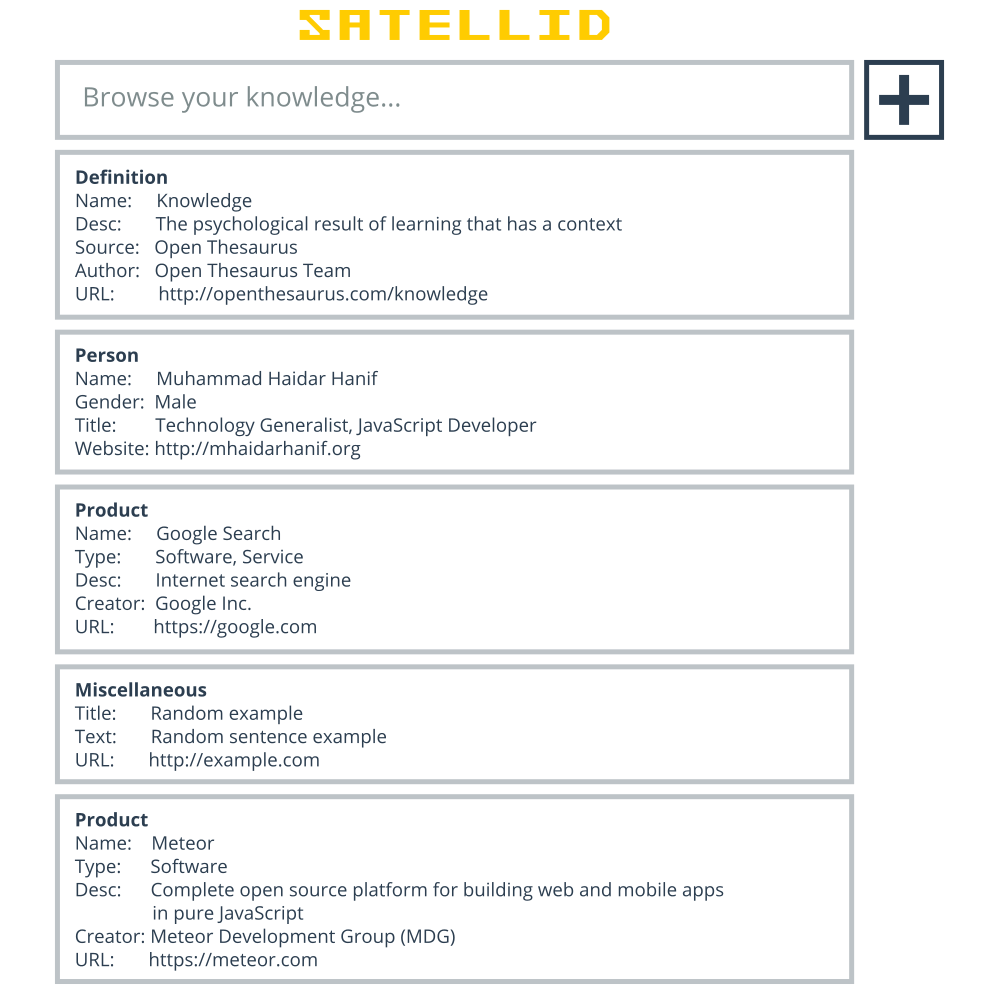
\includegraphics[height=10cm]{include/satellid-app-results_read.png}
    \vspace{-10pt}
    \label{fig:satellid-app-results_read}
  \end{figure}

\end{frame}

% ------------------------------------------------------------

\begin{frame}[fragile]
  \frametitle{App Result Screenshots: BROWSE}

  \begin{figure}[ht]
    \centering
    %TODO-SCREEN
    \vspace{-1cm}
    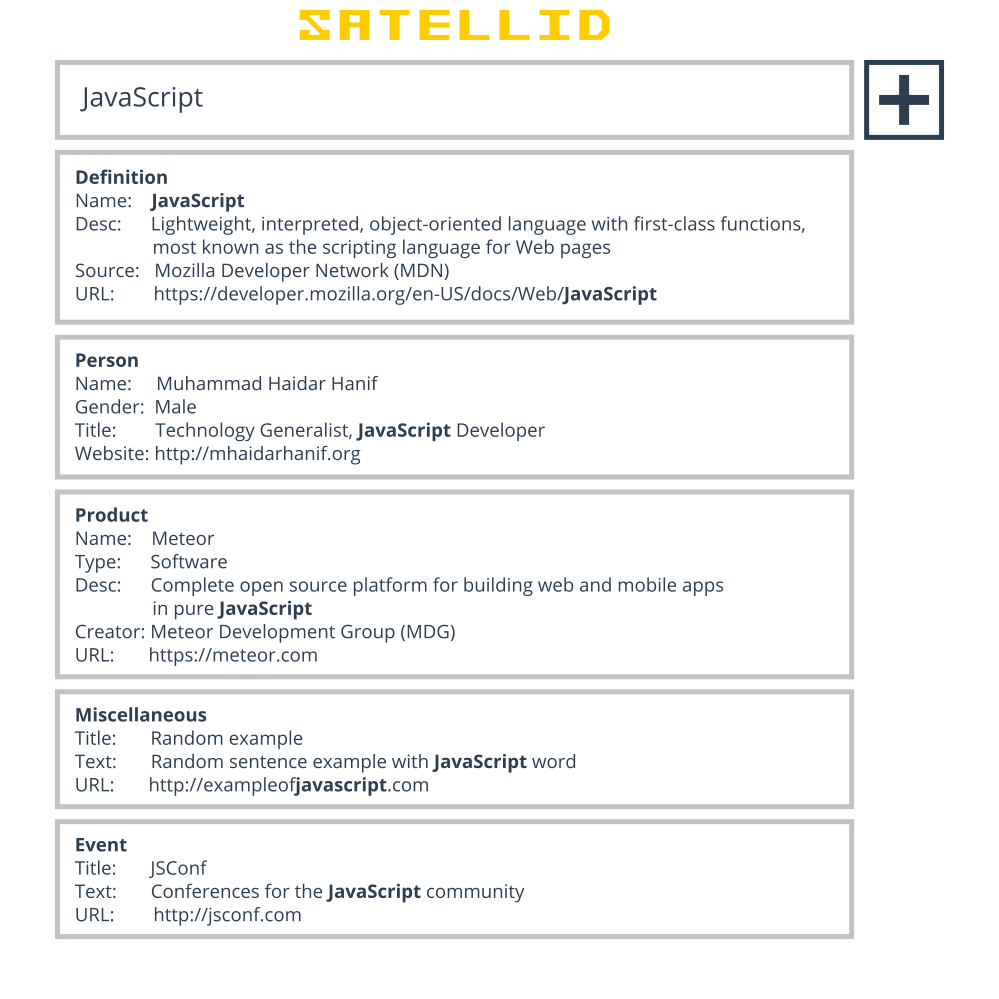
\includegraphics[height=10cm]{include/satellid-app-results_browse.png}
    \vspace{-10pt}
    \label{fig:satellid-app-results_browse}
  \end{figure}

\end{frame}

% ------------------------------------------------------------

\begin{frame}[fragile]
  \frametitle{App Result Screenshots: ADD}

  \begin{figure}[ht]
    \centering
    %TODO-SCREEN
    \vspace{-1cm}
    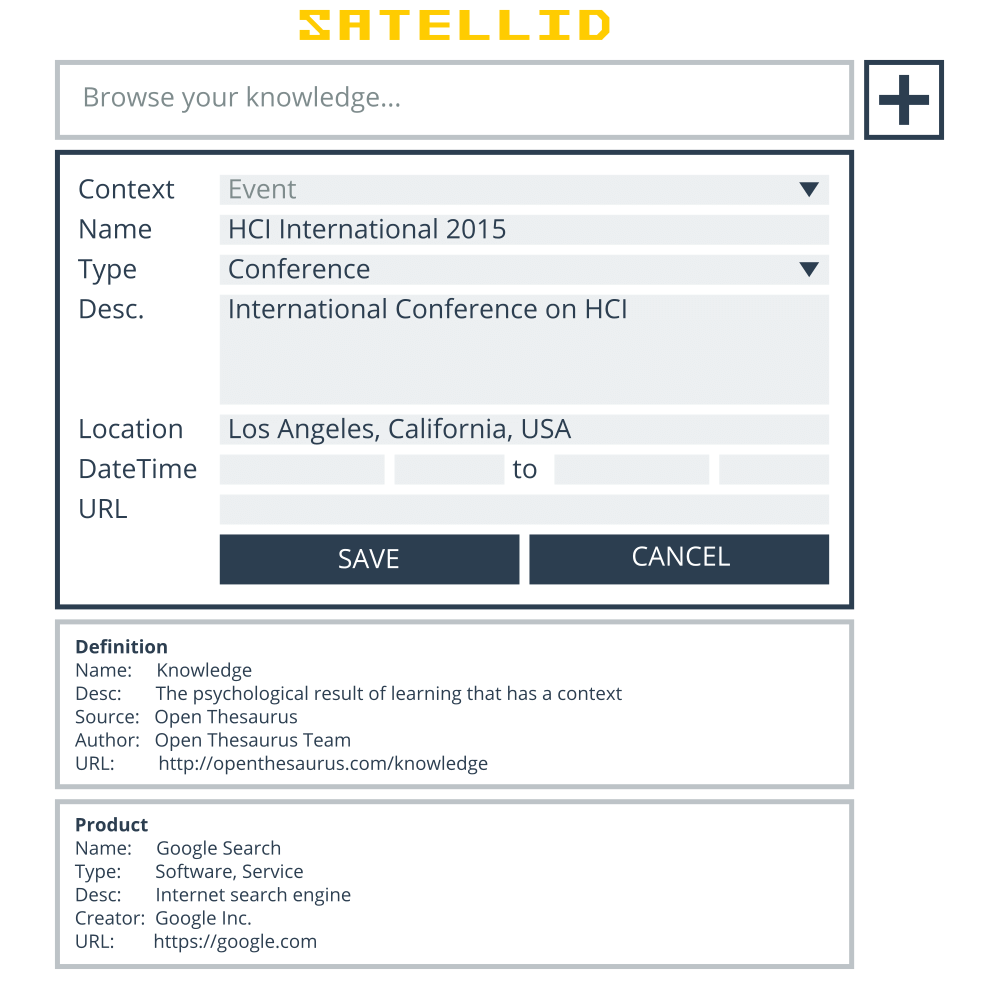
\includegraphics[height=10cm]{include/satellid-app-results_add.png}
    \vspace{-10pt}
    \label{fig:satellid-app-results_add}
  \end{figure}

\end{frame}

% ------------------------------------------------------------

\begin{frame}[fragile]
  \frametitle{App Result Screenshots: EDIT}

  \begin{figure}[ht]
    \centering
    %TODO-SCREEN
    \vspace{-1cm}
    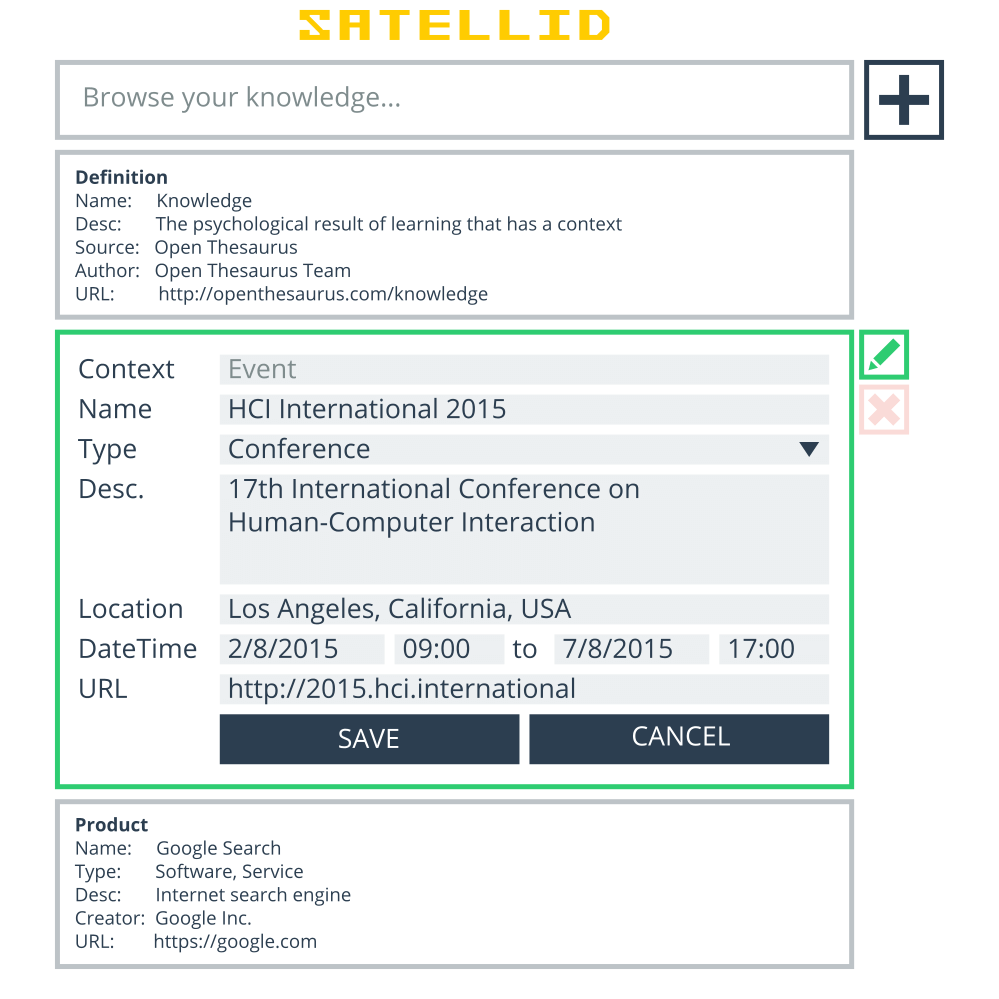
\includegraphics[height=10cm]{include/satellid-app-results_edit.png}
    \label{fig:satellid-app-results_edit}
  \end{figure}

\end{frame}

% ------------------------------------------------------------

\begin{frame}[fragile]
  \frametitle{App Result Screenshots: DELETE}

  \begin{figure}[ht]
    \centering
    %TODO-SCREEN
    \vspace{-1cm}
    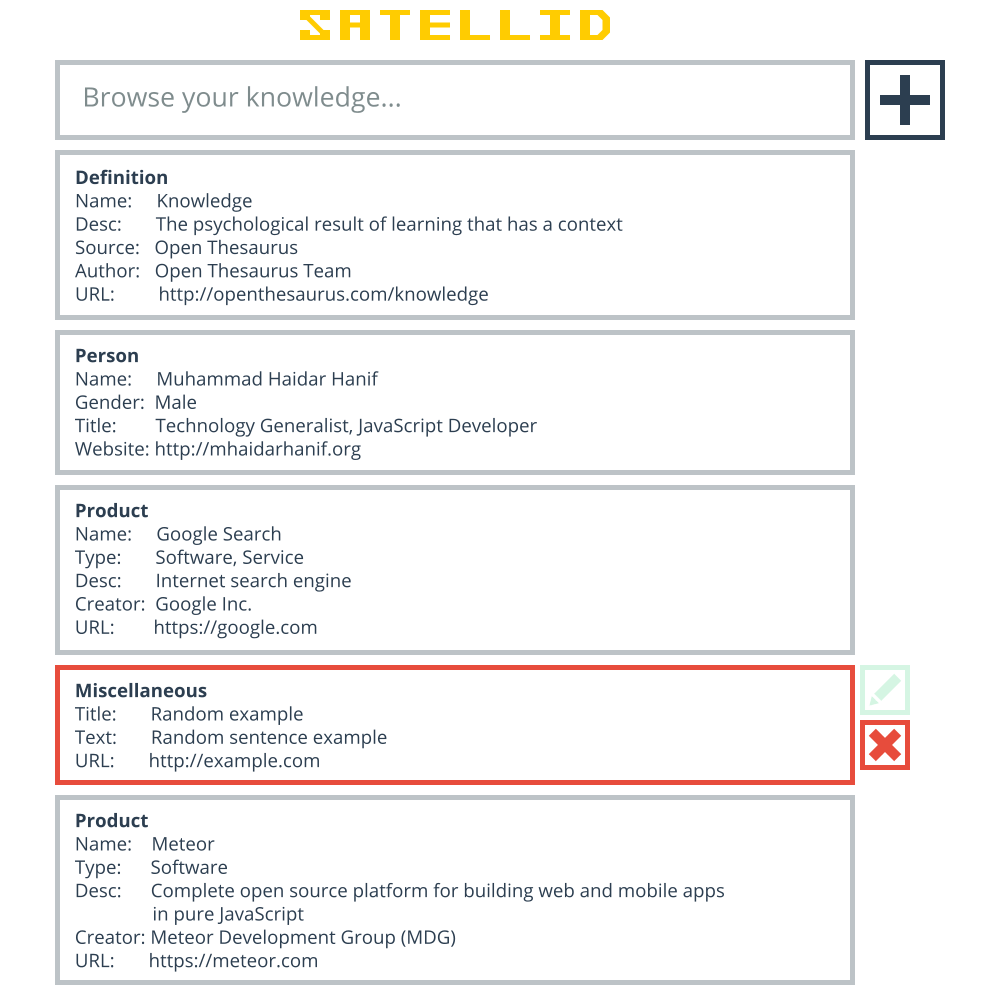
\includegraphics[height=10cm]{include/satellid-app-results_delete.png}
    \vspace{-10pt}
    \label{fig:satellid-app-results_delete}
  \end{figure}

\end{frame}

% ============================================================

\section{Closing}

% ------------------------------------------------------------

\begin{frame}[fragile]
  \frametitle{Conclusion}

  Simple and single \alert{system} of managing tons of \alert{personal daily knowledge}
  that implemented with \alert{Web technologies}

\end{frame}

% ------------------------------------------------------------

\begin{frame}[fragile]
  \frametitle{Suggestion}

  There could be some major issues, such as:

  \begin{itemize} \itemsep0pt
    \item There is no custom form yet.
    \item There is no easy way to import and export, including backup.
    % User start to use the app with a blank state, need to add all their present knowledge manually along the time.
  \end{itemize}

  So further and iterated improvement will remain to be done continuously.

\end{frame}

% ------------------------------------------------------------

\begin{frame}[fragile]
  \frametitle{Future Work}

  \begin{block}{Major}
    \begin{itemize} \itemsep0pt
      \item Can have custom form yet.
      \item Can easily import and export, even backup.
    \end{itemize}
  \end{block}

  \begin{block}{Others}
    Account system, more predefined context and field, \textsc{BREAD} the template, more custom configuration, multimedia support, integration with other networks, encryption, etc
  \end{block}

\end{frame}

% ============================================================

\plain{Thank You}

% ------------------------------------------------------------

\end{document}
